\documentclass[../documentacion_buscaminas2013.tex]{subfiles}
\begin{document}



\begin{figure}[!ht]
\paragraph{ } SCREENSHOTS

\paragraph{ } Ventana Inicial de nuestra aplicacionen la cual se presenta al usuario mientras se carga nuestra ventana principal del juego.
\newline
	~\newline
	\begin{center}
		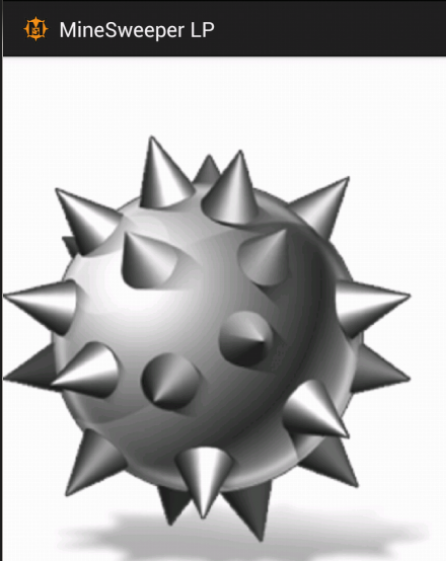
\includegraphics[width=0.5\textwidth]{./images/inicio.png}
	\end{center}
	%\caption{•}
	%\label{Figura 4.1}

~\newline
\paragraph{ } Luego que nuestra aplicacion ha cargado le presenta la ventana principal del juego en donde le mostramos tres opciones: Iniciar un nuevo juego, consultar los rankings del juego y una opcion acerca de los desarrolladores del juego.
\newline
	~\newline
	\begin{center}
		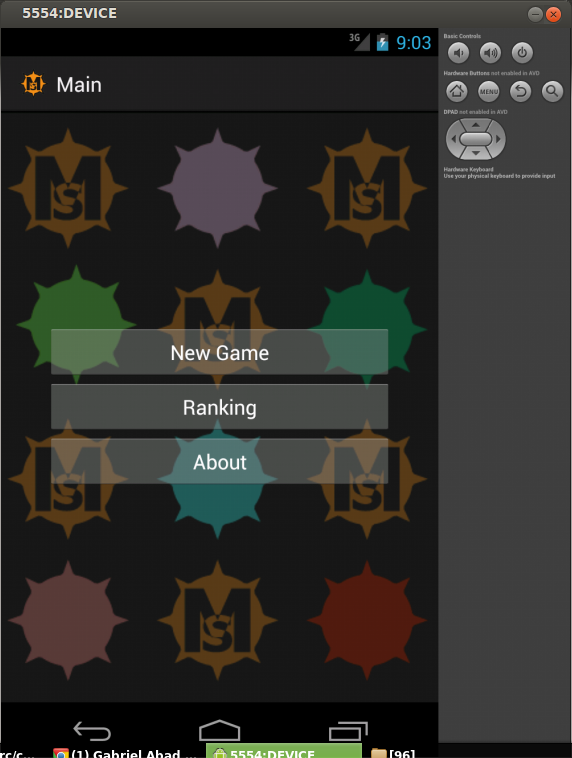
\includegraphics[width=0.5\textwidth]{./images/inicio2.png}
	\end{center}
	%\caption{•}
	%\label{Figura 4.2}
	
\end{figure}

\begin{figure}[!ht]
%\centering
\paragraph{ } Aqui mostramos los principales desarrolladores de la aplicacion.
\newline
	~\newline
	\begin{center}
		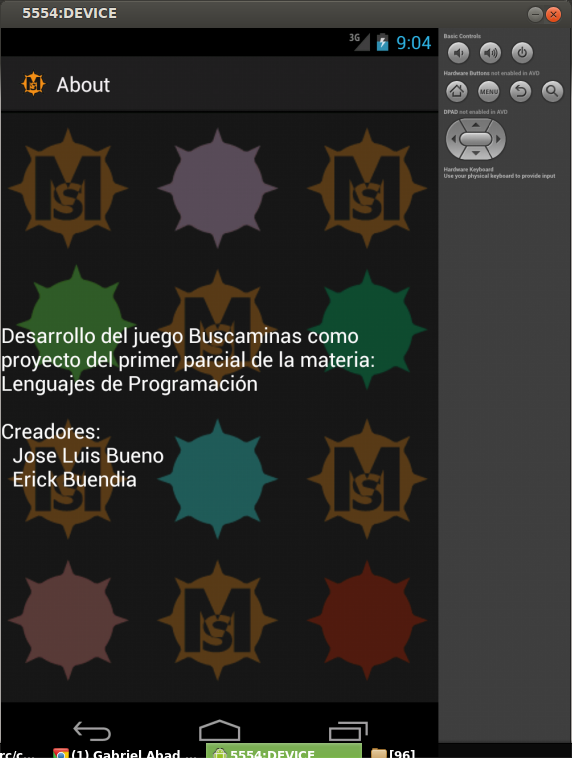
\includegraphics[width=0.5\textwidth]{./images/about.png}
	\end{center}
	%\caption{•}
	%\label{Figura 4.3}

~\newline
\paragraph{ } Vista de tablero implementado en la aplicacion que dispone de un determinado numero de casillas dependiendo del nivel escogido por el usuario y de un contador que sirve para el manejo del ranking.
\newline
	~\newline
	\begin{center}
		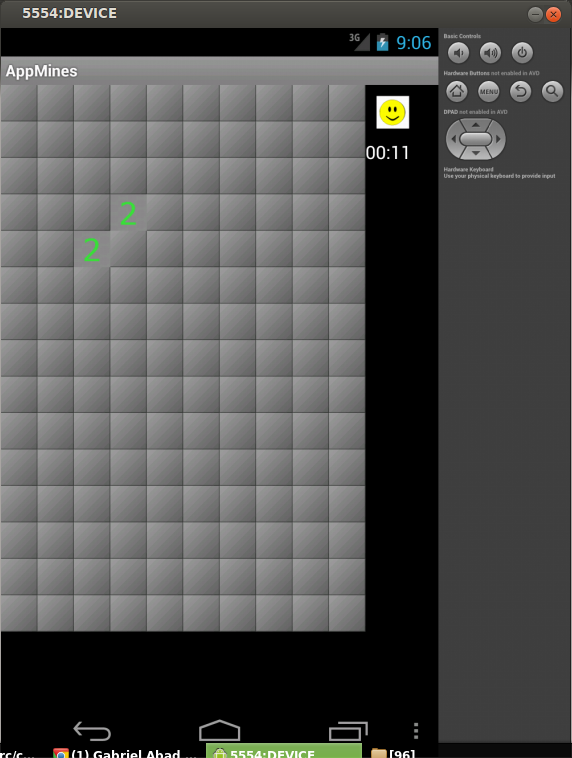
\includegraphics[width=0.5\textwidth]{./images/tablero.png}
	\end{center}
	%\caption{•}
	%\label{Figura 4.4}

\end{figure}

\begin{figure}[!ht]
%\centering
\paragraph{ } Pantalla que muestra los puntajes de los usuarios de la aplicacion.
\newline
	~\newline
	\begin{center}
		
\includegraphics[width=0.5\textwidth]{./images/ranking.png}
	\end{center}
	%\caption{•}
	%\label{Figura 4.5}

~\newline
\paragraph{ } Pantalla que muestra el nivel facil del juego. Tablero de 8x8.
\newline
	~\newline
	\begin{center}
		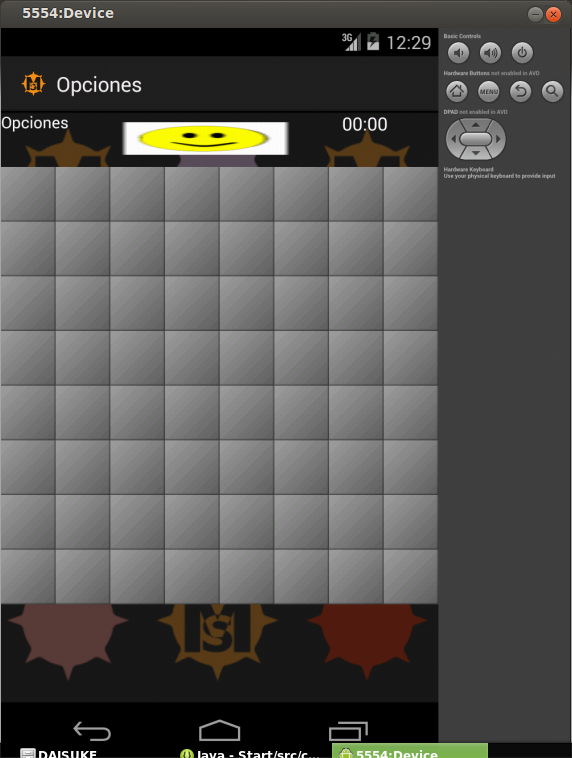
\includegraphics[width=0.5\textwidth]{./images/facil.png}
	\end{center}
	%\caption{•}
	%\label{Figura 4.6}

\end{figure}

\begin{figure}[!ht]
%\centering
\paragraph{ }  Pantalla que muestra el nivel medio del juego. Tablero de 16x16
\newline
	~\newline
	\begin{center}
		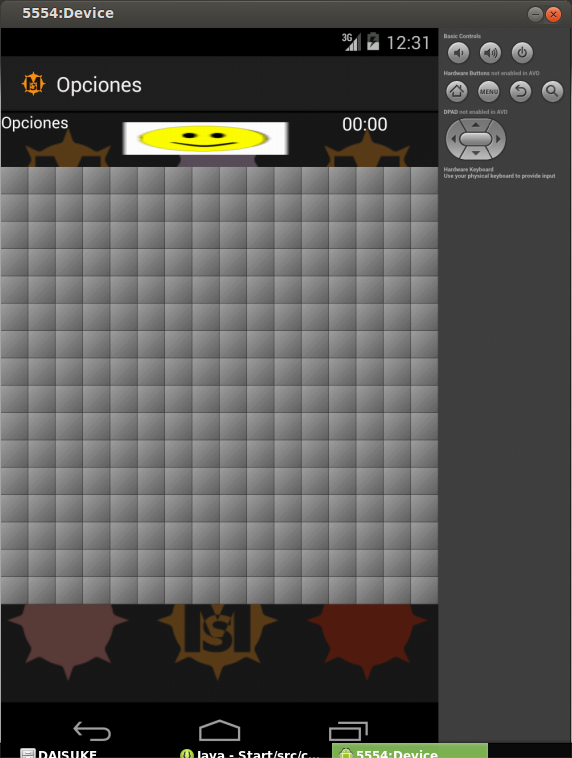
\includegraphics[width=0.5\textwidth]{./images/medio.png}
	\end{center}
	%\caption{•}
	%\label{Figura 4.7}

~\newline
\paragraph{ }  Pantalla que muestra el nivel avanzado del juego. Tablero de 30x16
\newline
	~\newline
	\begin{center}
		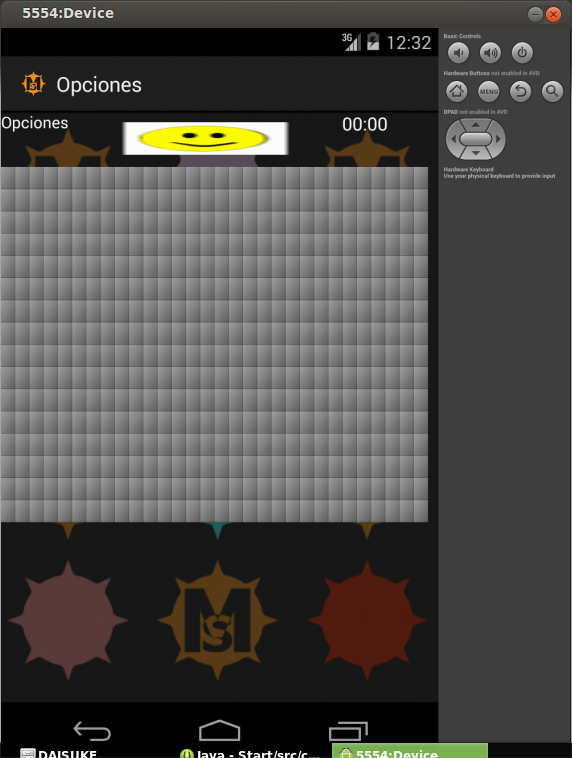
\includegraphics[width=0.5\textwidth]{./images/avanzado.png}
	\end{center}
	
	%\caption{•}
	%\label{Figura 4.8}

\end{figure}


\clearpage
\end{document}
